%% Copernicus Publications Manuscript Preparation Template for LaTeX Submissions
%% ---------------------------------
%% This template should be used for copernicus.cls
%% The class file and some style files are bundled in the Copernicus Latex Package, which can be downloaded from the different journal webpages.
%% For further assistance please contact Copernicus Publications at: production@copernicus.org
%% https://publications.copernicus.org/for_authors/manuscript_preparation.html


%% Please use the following documentclass and journal abbreviations for preprints and final revised papers.

%% 2-column papers and preprints
\documentclass[esd, article]{copernicus}



%% Journal abbreviations (please use the same for preprints and final revised papers)


% Advances in Geosciences (adgeo)
% Advances in Radio Science (ars)
% Advances in Science and Research (asr)
% Advances in Statistical Climatology, Meteorology and Oceanography (ascmo)
% Annales Geophysicae (angeo)
% Archives Animal Breeding (aab)
% ASTRA Proceedings (ap)
% Atmospheric Chemistry and Physics (acp)
% Atmospheric Measurement Techniques (amt)
% Biogeosciences (bg)
% Climate of the Past (cp)
% DEUQUA Special Publications (deuquasp)
% Drinking Water Engineering and Science (dwes)
% Earth Surface Dynamics (esurf)
% Earth System Dynamics (esd)
% Earth System Science Data (essd)
% E&G Quaternary Science Journal (egqsj)
% European Journal of Mineralogy (ejm)
% Fossil Record (fr)
% Geochronology (gchron)
% Geographica Helvetica (gh)
% Geoscience Communication (gc)
% Geoscientific Instrumentation, Methods and Data Systems (gi)
% Geoscientific Model Development (gmd)
% History of Geo- and Space Sciences (hgss)
% Hydrology and Earth System Sciences (hess)
% Journal of Bone and Joint Infection (jbji)
% Journal of Micropalaeontology (jm)
% Journal of Sensors and Sensor Systems (jsss)
% Magnetic Resonance (mr)
% Mechanical Sciences (ms)
% Natural Hazards and Earth System Sciences (nhess)
% Nonlinear Processes in Geophysics (npg)
% Ocean Science (os)
% Polarforschung - Journal of the German Society for Polar Research (polf)
% Primate Biology (pb)
% Proceedings of the International Association of Hydrological Sciences (piahs)
% Scientific Drilling (sd)
% SOIL (soil)
% Solid Earth (se)
% The Cryosphere (tc)
% Weather and Climate Dynamics (wcd)
% Web Ecology (we)
% Wind Energy Science (wes)


%% \usepackage commands included in the copernicus.cls:
%\usepackage[german, english]{babel}
%\usepackage{tabularx}
%\usepackage{cancel}
%\usepackage{multirow}
%\usepackage{supertabular}
%\usepackage{algorithmic}
%\usepackage{algorithm}
%\usepackage{amsthm}
%\usepackage{float}
%\usepackage{subfig}
%\usepackage{rotating}


\begin{document}

\title{Potential for bias in effective climate sensitivity from state-dependent energetic balance}


% \Author[affil]{given_name}{surname}

\Author[1]{Benjamin M.}{Sanderson}
\Author[2]{Maria}{Rugenstein}


\affil[1]{CERFACS, Toulouse, France}
\affil[2]{Colorado State University, Fort Collins CO, USA}



\correspondence{Benjamin Sanderson (sanderson@cerfacs.fr)}

\runningtitle{state-dependent energetic balance}

\runningauthor{Sanderson et al.}





\received{}
\pubdiscuss{} %% only important for two-stage journals
\revised{}
\accepted{}
\published{}

%% These dates will be inserted by Copernicus Publications during the typesetting process.


\firstpage{1}

\maketitle



\begin{abstract}
Model estimates of equilibrium climate sensitivity are generally approximated from tendencies in 150  year simulations, given full equilibration occurs on timescales of millennia.  Estimates are made by linear extrapolation of temperature as a function of top of atmosphere energetic imbalance to estimate the temperature change in an equilibrated state.  In this study, we consider an alternative approach for estimating ECS through Bayesian calibration of a multiple timescale response model.  Though the method leaves large uncertainties in ECS using conventional 150 year CO2 quadrupling experiments, application to millennial timescale experiments suggests potential biases in EffCS in the case of particular models where the equilibrium energetic state of the model differs between the pre-industrial and quadrupled CO2 states.  These biases may imply a reconsideration of certain CMIP6 model climate sensitivities, potentially ruling out models which exhibited high climate sensitivity and low transient climate response. 
\end{abstract}


%\copyrightstatement{TEXT} %% This section is optional and can be used for copyright transfers.


\introduction  
Equilibrium Climate Sensitivity (ECS) of an Earth System Model is the equilibrium increase in global mean temperature experienced in response to an instantaneous doubling change in carbon dioxide concentrations.  Introduced as a metric of response of the Earth System to greenhouse gases in the early years of computational climate science \citep{charney1979carbon,hansen1984climate}, it remains a very common metric of the sensitivity of the Earth to greenhouse gas forcing \cite{knutti2017beyond,stocker2013climate}.

Measuring ECS in a coupled climate model, however, is difficult owing to the time required for the equilibration of the system to a change in forcing \cite{wetherald2001committed,solomon2010persistence,jarvis2011contribution}. necessitating simulations of multiple millennia to obtain a near-equilibrated estimate of temperature response \cite{rugenstein2020equilibrium}.  The computational burden of conducting such simulations implies that standard practise for model assessment \citep{stocker2013climate,forster2016inference,andrews2012forcing} is to measure an "Effective Climate Sensitivity" (EffCS) using feedbacks extrapolated from those measures in the first 150 years of a quadrupled CO$_2$ simulation \cite{gregory2004new,murphy1995transient}.

Recent work, however, has highlighted potential uncertainties in the EffCS approximation of ECS - studies have found that net radiative feedbacks can exhibit both timescale dependencies \cite{proistosescu2017slow,andrews2018accounting} and state dependencies \citep{pfister2017state,bloch2021climate} both of which draw into question the implicit constant feedback assumption used in the derivation of EffCS.

The LongrunMIP project set out to quantify this error by running a subset of Earth System Models in idealised carbon dioxide perturbation experiments with simulations of millennial timescale response \citep{rugenstein2019longrunmip}.  Initial studies compared the EffCS as derived using the first 150 years of the simulation with that derived using the last 15 percent of warming in multi-thousand year experiments - finding that the accuracy of the EffCS varied by model, but in most cases represented a 10$\%$ error or less in the estimate of ECS \cite{rugenstein2020equilibrium}.

A general assessment of the likely range of EffCS \citep{sherwood2020assessment} explicitly requires prior assumptions on the ratio of ECS:EffCS (represented by a parameter $\zeta$ such that ECS/EffCS is given by $(1+\zeta)$), given that the confidence in headline upper bound of EffCS in the study rests on combined evidence of paleo evidence and recent historical evidence.  The paleo evidence represents the near-equilibrium response, so prior confidence that $\zeta$ is small, itself arising from LongrunMIP \citep{rugenstein2020equilibrium}, contributes to the headline result that values of EffCS of greater than 4.5K are unlikely.

The findings of \cite{sherwood2020assessment} somewhat challenge the use of the CMIP6 ensemble of climate models \citep{eyring2016overview} as a proxy for climate projection uncertainty in assessment \citep{o2016scenario}, given approximately 1/3 of the ensemble \citep{meehl2020context} have EffCS values of greater than  4.7K (the 95th percentile of the distribution as assessed by \cite{sherwood2014spread}).  The high EffCS values in CMIP6 have been attributed to stronger positive cloud feedbacks \cite{zelinka2020causes}.  

So how plausible are the higher sensitivity models?  Studies have found that one of the higher sensitivity models (CESM2) tend to perform more poorly in paleoclimate simulations than its lower sensitivity predecessors \citep{zhu2020high}.  Although studies \citep{nijsse2020emergent,tokarska2020past} suggest that post-1980 warming may help constrain the Transient Climate Response (the warming expected at time of CO$_2$ doubling in an experiment with a 1 percent annual concentration increase), the constrain on EffCS from historical warming alone is weaker both in terms of correlations in the CMIP ensemble \cite{tokarska2018cumulative} and in ensembles of simple models \cite{sanderson2020relating,sherwood2020assessment}.

A core assumption in the calculation of EffCS is that the system will ultimately stabilise in a state of energetic balance \cite{gregory2004new}.  However, in practise a number of models exhibit energetic radiative top of atmosphere imbalances in the control state \cite{rugenstein2019longrunmip}, and as such the Effective Climate Sensitivity is calculated using net fluxes relative to the control mean top of atmosphere net radiative fluxes.  However, it remains untested as to whether such models will ultimately converge to the same state of imbalance.

In the present study, we consider an alternative approach for calculating climate sensitivity from a climate simulation in which there is a step change in carbon dioxide concentrations.  We consider how the method of calculating effective climate sensitivity, either from initial response or from millennial scale simulations, may be potentially subject to biases arising from assumptions on the equilibrated radiative state.  Finally, we consider how these uncertainties may relate to our confidence in the relationship between climate feedbacks on the post-industrial and paleoclimate timescales.

\section{Methods}
We consider available pre-industrial control simulations (PiCTRL) and abrupt CO2 quadrupling experiments (4xCO2) from 3 available ensembles: CMIP5 \citep{taylor2012overview}, CMIP6 \citep{eyring2016overview} and LongRunMIP \cite{rugenstein2019longrunmip}.  From each of these, we compute global averages of surface temperature, plus top of atmosphere shortwave and longwave fluxes.

We assume that the temperature and radiative timeseries can be modelled by a sum of exponential decay terms, a basis set \cite{proistosescu2017slow,sanderson2020relating} which is consistent with the general solution of two layer simple climate models with \cite{geoffroy2013transient,winton2010importance,smith2018fair} or without \cite{geoffroy2013constant} terms for ocean heat uptake efficacy.  

As in \cite{proistosescu2017slow}, we allow for three independent equilibration timescales, such that:


\begin{align}
   T(t)&=\sum_{n=1}^3 S_n(1-e^{-(t/\tau_n)})+T_0\\
   R(t)&=\sum_{n=1}^3 R_n(-e^{-(t/\tau_n)})+R_0.
\label{eq1}
\end{align}

Where $T(t)$ and $R(t)$ are the global annual mean surface temperature and net top of atmosphere radiative flux timeseries respectively, $tau_n$ is the decay time associated with the timescale $n$, $S_n$ and $R_n$ are scaling factors and $T_0$ and $R_0$ are constant terms. $T_0$ is taken as the mean temperature in the last available 500 years of the control simulation.  $R_0$ represents the radiative flux imbalance at an infinite time, and is calibrated during the analysis.  In models with no energetic leaks, $R_0=0$, but this is not always the case and small energetic imbalances remain in some models even after the model global mean temperature trends have ceased \citep{rugenstein2019longrunmip}.

\subsection{Bayesian Calibration of long term response parameters}
We fit the response equations detailed in \ref{eq1} to the output of each ensemble member's global mean radiative flux and surface temperature timeseries using a Markov Chain Monte Carlo optimizer \cite{foreman2013emcee} (as implemented in the 'lmfit' Python module), allowing for $n=3$ representative decay timescales.  Parameter ranges are constrained according to Table \ref{tb1}.  

\begin{table}[]
    \centering
    \begin{tabular}{l|l|l|c|c}
    Parameter & long name & Units & Min value & Max value \\
    $S_1$ & Short timescale sensitivity & K & 0 & 10 \\
    $S_2$ & Intermediate timescale sensitivity & K & 0 & 10 \\
    $S_3$ & Long timescale sensitivity & K & 0 & 10 \\
    $\tau_1$ & Short timescale & years & 0 & 10 \\
    $\tau_2$ & Intermediate timescale & years & 100 & 150 \\
    $\tau_3$ & Long timescale & years & 150 & 2000 \\
    $R_0$ & Equilibrium energy leak & Wm$^{-2}$ & -5 & 5 \\
    \end{tabular}
    \caption{Parameters and prior ranges considered in the Bayesian calibration of equation \ref{eq1}}
    \label{tab:my_label}
\end{table}

The results for the fitted exponential models for 4xCO2 simulations in the LongRunMIP archive are presented in Figure \ref{fig:greg_lrmip}.  

\begin{figure}
    \centering
    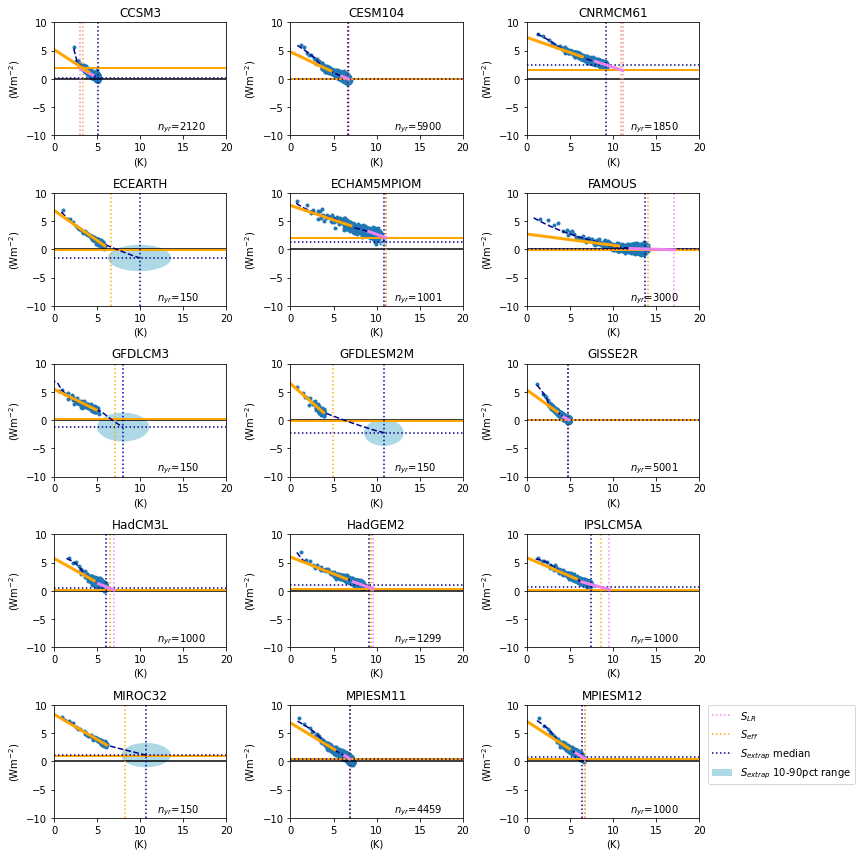
\includegraphics[width=\linewidth]{greg_lrmip.png}
    \caption{An illustration of the }
    \label{fig:greg_lrmip}
\end{figure}


\subsection{HEADING}
TEXT


\subsubsection{HEADING}
TEXT


\conclusions  %% \conclusions[modified heading if necessary]
TEXT

%% The following commands are for the statements about the availability of data sets and/or software code corresponding to the manuscript.
%% It is strongly recommended to make use of these sections in case data sets and/or software code have been part of your research the article is based on.

\codeavailability{TEXT} %% use this section when having only software code available


\dataavailability{TEXT} %% use this section when having only data sets available


\codedataavailability{TEXT} %% use this section when having data sets and software code available


\sampleavailability{TEXT} %% use this section when having geoscientific samples available


\videosupplement{TEXT} %% use this section when having video supplements available


\appendix
\section{}    %% Appendix A

\subsection{}     %% Appendix A1, A2, etc.


\noappendix       %% use this to mark the end of the appendix section. Otherwise the figures might be numbered incorrectly (e.g. 10 instead of 1).

%% Regarding figures and tables in appendices, the following two options are possible depending on your general handling of figures and tables in the manuscript environment:

%% Option 1: If you sorted all figures and tables into the sections of the text, please also sort the appendix figures and appendix tables into the respective appendix sections.
%% They will be correctly named automatically.

%% Option 2: If you put all figures after the reference list, please insert appendix tables and figures after the normal tables and figures.
%% To rename them correctly to A1, A2, etc., please add the following commands in front of them:

\appendixfigures  %% needs to be added in front of appendix figures

\appendixtables   %% needs to be added in front of appendix tables

%% Please add \clearpage between each table and/or figure. Further guidelines on figures and tables can be found below.



\authorcontribution{TEXT} %% this section is mandatory

\competinginterests{TEXT} %% this section is mandatory even if you declare that no competing interests are present

\disclaimer{TEXT} %% optional section

\begin{acknowledgements}
TEXT
\end{acknowledgements}




\bibliographystyle{copernicus}
\bibliography{sample_full.bib}


\end{document}
